


\tikzset{every picture/.style={line width=0.75pt}} %set default line width to 0.75pt        

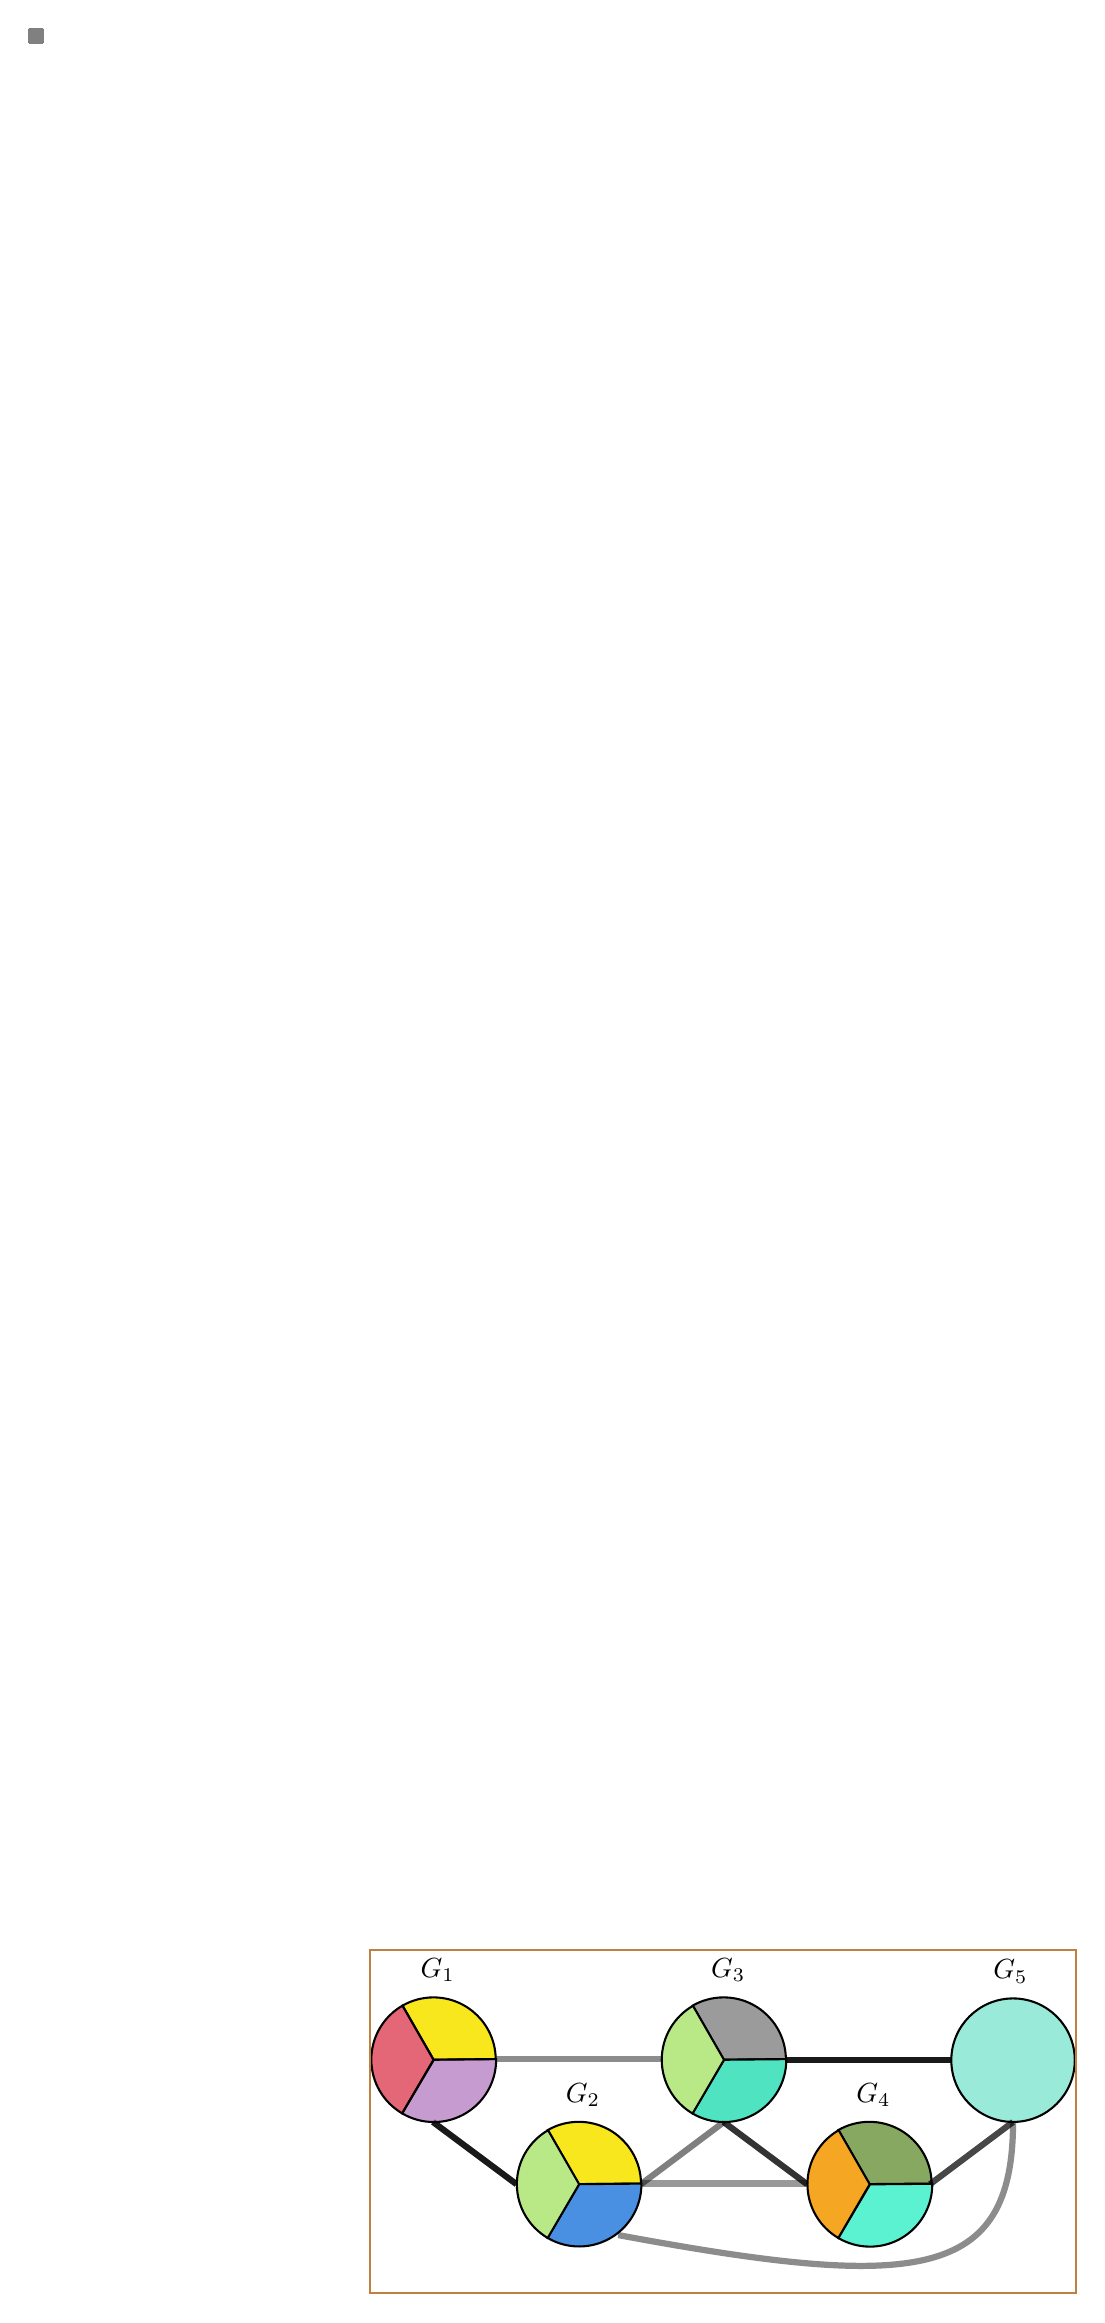
\begin{tikzpicture}[x=0.75pt,y=0.75pt,yscale=-1,xscale=1]
%uncomment if require: \path (0,1438); %set diagram left start at 0, and has height of 1438

%Straight Lines [id:da6191954638465524] 
\draw [color={rgb, 255:red, 0; green, 0; blue, 0 }  ,draw opacity=0.9 ][line width=2.25]    (190.75,1005.5) -- (231,1035.5) ;
%Straight Lines [id:da10859841922747804] 
\draw [color={rgb, 255:red, 0; green, 0; blue, 0 }  ,draw opacity=0.5 ][line width=2.25]    (291,1035.5) -- (331,1005.5) ;
%Straight Lines [id:da9227391972497354] 
\draw [color={rgb, 255:red, 0; green, 0; blue, 0 }  ,draw opacity=0.8 ][line width=2.25]    (330.75,1005.5) -- (371,1035.5) ;
%Straight Lines [id:da300768104867311] 
\draw [color={rgb, 255:red, 0; green, 0; blue, 0 }  ,draw opacity=0.9 ][line width=2.25]    (360.5,975.75) -- (440.5,975.75) ;
%Shape: Pie [id:dp9639779729779112] 
\draw  [fill={rgb, 255:red, 248; green, 231; blue, 28 }  ,fill opacity=1 ] (176.1,949.46) .. controls (180.49,946.94) and (185.58,945.5) .. (191,945.5) .. controls (207.48,945.5) and (220.86,958.79) .. (221,975.23) -- (191,975.5) -- cycle ;
%Shape: Pie [id:dp5221762953249574] 
\draw  [fill={rgb, 255:red, 170; green, 106; blue, 183 }  ,fill opacity=0.67 ] (221.19,975.25) .. controls (221.19,975.35) and (221.19,975.45) .. (221.19,975.55) .. controls (221.19,992.11) and (207.76,1005.55) .. (191.19,1005.55) .. controls (185.62,1005.55) and (180.39,1004.02) .. (175.92,1001.37) -- (191.19,975.55) -- cycle ;
%Shape: Pie [id:dp2628811822033663] 
\draw  [fill={rgb, 255:red, 208; green, 2; blue, 27 }  ,fill opacity=0.6 ] (175.92,1001.37) .. controls (167.03,996.17) and (161.06,986.51) .. (161.06,975.47) .. controls (161.06,964.35) and (167.11,954.64) .. (176.1,949.46) -- (191.06,975.47) -- cycle ;
%Shape: Pie [id:dp6613907142053934] 
\draw  [fill={rgb, 255:red, 155; green, 155; blue, 155 }  ,fill opacity=1 ] (315.9,949.46) .. controls (320.29,946.94) and (325.38,945.5) .. (330.81,945.5) .. controls (347.29,945.5) and (360.66,958.79) .. (360.8,975.23) -- (330.81,975.5) -- cycle ;
%Shape: Pie [id:dp4276424084769457] 
\draw  [fill={rgb, 255:red, 80; green, 227; blue, 194 }  ,fill opacity=1 ] (361,975.25) .. controls (361,975.35) and (361,975.45) .. (361,975.55) .. controls (361,992.11) and (347.57,1005.55) .. (331,1005.55) .. controls (325.42,1005.55) and (320.2,1004.02) .. (315.73,1001.37) -- (331,975.55) -- cycle ;
%Shape: Pie [id:dp906360766003214] 
\draw  [fill={rgb, 255:red, 184; green, 233; blue, 134 }  ,fill opacity=1 ] (315.86,1001.45) .. controls (306.97,996.25) and (301,986.59) .. (301,975.55) .. controls (301,964.43) and (307.05,954.72) .. (316.04,949.54) -- (331,975.55) -- cycle ;
%Shape: Pie [id:dp7403887775524796] 
\draw  [fill={rgb, 255:red, 65; green, 117; blue, 5 }  ,fill opacity=0.63 ] (386.1,1009.41) .. controls (390.49,1006.89) and (395.58,1005.45) .. (401,1005.45) .. controls (417.48,1005.45) and (430.86,1018.74) .. (431,1035.19) -- (401,1035.45) -- cycle ;
%Shape: Pie [id:dp8013437505172472] 
\draw  [fill={rgb, 255:red, 90; green, 242; blue, 208 }  ,fill opacity=1 ] (431.33,1035.29) .. controls (431.33,1035.38) and (431.33,1035.48) .. (431.33,1035.58) .. controls (431.33,1052.15) and (417.9,1065.58) .. (401.33,1065.58) .. controls (395.75,1065.58) and (390.53,1064.06) .. (386.06,1061.41) -- (401.33,1035.58) -- cycle ;
%Shape: Pie [id:dp5376876560242096] 
\draw  [fill={rgb, 255:red, 245; green, 166; blue, 35 }  ,fill opacity=1 ] (386.06,1061.41) .. controls (377.17,1056.2) and (371.19,1046.55) .. (371.19,1035.5) .. controls (371.19,1024.38) and (377.24,1014.67) .. (386.23,1009.49) -- (401.19,1035.5) -- cycle ;
%Shape: Pie [id:dp9239995069986118] 
\draw  [fill={rgb, 255:red, 248; green, 231; blue, 28 }  ,fill opacity=1 ] (246.1,1009.41) .. controls (250.49,1006.89) and (255.58,1005.45) .. (261,1005.45) .. controls (277.48,1005.45) and (290.86,1018.74) .. (291,1035.19) -- (261,1035.45) -- cycle ;
%Shape: Pie [id:dp5557360553254671] 
\draw  [fill={rgb, 255:red, 74; green, 144; blue, 226 }  ,fill opacity=1 ] (291.19,1035.21) .. controls (291.19,1035.3) and (291.19,1035.4) .. (291.19,1035.5) .. controls (291.19,1052.07) and (277.76,1065.5) .. (261.19,1065.5) .. controls (255.62,1065.5) and (250.39,1063.98) .. (245.92,1061.33) -- (261.19,1035.5) -- cycle ;
%Shape: Pie [id:dp7328167973725814] 
\draw  [fill={rgb, 255:red, 184; green, 233; blue, 134 }  ,fill opacity=1 ] (246.06,1061.41) .. controls (237.17,1056.2) and (231.19,1046.55) .. (231.19,1035.5) .. controls (231.19,1024.38) and (237.24,1014.67) .. (246.23,1009.49) -- (261.19,1035.5) -- cycle ;
%Shape: Circle [id:dp18652142322857346] 
\draw  [fill={rgb, 255:red, 153; green, 234; blue, 216 }  ,fill opacity=1 ] (440.5,975.75) .. controls (440.5,959.32) and (453.82,946) .. (470.25,946) .. controls (486.68,946) and (500,959.32) .. (500,975.75) .. controls (500,992.18) and (486.68,1005.5) .. (470.25,1005.5) .. controls (453.82,1005.5) and (440.5,992.18) .. (440.5,975.75) -- cycle ;
%Straight Lines [id:da8957245080676144] 
\draw [color={rgb, 255:red, 0; green, 0; blue, 0 }  ,draw opacity=0.45 ][line width=2.25]    (221.19,975.25) -- (301.19,975.25) ;
%Straight Lines [id:da4142437492290467] 
\draw [color={rgb, 255:red, 0; green, 0; blue, 0 }  ,draw opacity=0.72 ][line width=2.25]    (430.25,1035.5) -- (470.25,1005.5) ;
%Straight Lines [id:da5271159074032483] 
\draw [color={rgb, 255:red, 0; green, 0; blue, 0 }  ,draw opacity=0.4 ][line width=2.25]    (291.19,1035.21) -- (371.19,1035.21) ;
%Curve Lines [id:da5911048150718752] 
\draw [color={rgb, 255:red, 0; green, 0; blue, 0 }  ,draw opacity=0.45 ][line width=2.25]    (280,1060) .. controls (423.2,1086.6) and (470.2,1082.6) .. (470.25,1005.5) ;

% Text Node
\draw (193,932.5) node   [align=left] {$\displaystyle G_{1}$};
% Text Node
\draw (263,992.5) node   [align=left] {$\displaystyle G_{2}$};
% Text Node
\draw (333,932.5) node   [align=left] {$\displaystyle G_{3}$};
% Text Node
\draw (403,992.5) node   [align=left] {$\displaystyle G_{4}$};
% Text Node
\draw (469,933.08) node   [align=left] {$\displaystyle G_{5}$};

\draw [brown] (current bounding box.south west) rectangle (current bounding box.north east);

\draw[gray,step=0.25] (-4,-3) grid (3, 4);
\end{tikzpicture}